\documentclass[autodetect-engine,dvipdfmx-if-dvi,ja=standard,everyparhook=compat]{bxjsarticle}

\usepackage{graphicx}        % 図を表示するのに必要
\usepackage{color}           % jpgなどを表示するのに必要
\usepackage{amsmath,amssymb} % 数学記号を出すのに必要
\usepackage{type1cm}         % fontsizeのエラー回避
\usepackage{here}            % 図の強制配置
\usepackage{url}             % URLをいい感じにしてくれる
\usepackage{subfigure}       % 図をまとめて表示
\usepackage{pdfpages}        % PDFの連結
\usepackage{setspace}
\usepackage{cases}
\usepackage{fancyhdr}
\usepackage{wrapfig}% 図の回り込み


% 余白の設定
% \setlength{\textheight}{\paperheight}   % 紙面縦幅を本文領域にする(BOTTOM=-TOP)
% \setlength{\topmargin}{-15.4truemm}     % 上の余白を10mm(=1inch-15.4mm)に
% \addtolength{\topmargin}{-\headheight}  %
% \addtolength{\topmargin}{-\headsep}     % ヘッダの分だけ本文領域を移動させる
% \addtolength{\textheight}{-20truemm}    % 下の余白も10mm
% \setlength{\textwidth}{\paperwidth}     % 紙面横幅を本文領域にする(RIGHT=-LEFT)
% \setlength{\oddsidemargin}{-5.4truemm}  % 奇数ページの左の余白を20mm(=1inch-5.4mm)に
% \setlength{\evensidemargin}{-5.4truemm} % 偶数数ページの左の余白を20mm(=1inch-5.4mm)に
% \addtolength{\textwidth}{-40truemm}     % 右の余白も20mm

% タイトル
\title{タイトル}

% ヘッダとフッタの設定
% \lhead{電気電子情報工学実験}
% \chead{}
% \rhead{20315784 佐藤凌雅}
% \lfoot{}
% \cfoot{\thepage} % ページ数
% \rfoot{}

\parindent = 0pt  % 行頭の字下げをしない
\setstretch{1.0}  % 行間

% キャプションの英語化
\renewcommand{\figurename}{Fig.}
\renewcommand{\tablename}{Table}

% 各章,節などタイトルの大きさを変更
% \titleformat*{\section}{\Huge\bfseries}
% \titleformat*{\subsection}{\Large\bfseries}

% 式の番号を(senction_num.num)のようにする
% \makeatletter
% \@addtoreset{equation}{chapter}
% \def\theequation{\thechapter.\arabic{equation}}
% \makeatother

% 呼び出したページのページ番号を消す
\newcommand{\deletePageNum}{
    \thispagestyle{empty}
    \clearpage
    \addtocounter{page}{-1}
}

% urlのフォントを直す
\renewcommand\UrlFont{\rmfamily}


\begin{document}
\fontsize{14.041pt}{18.562pt}\selectfont
\begin{center}
    \textbf{
    電気電子情報工学実験I「サーボモータの制御」レポート課題\\
    電気電子情報工学課程 3年 20315784 佐藤凌雅\\
    }
\end{center}

\fontsize{11.041pt}{16.562pt}\selectfont

\section{課題1:今日の講義内容を「自分の言葉で!」まとめよ.}
\subsection{はじめに}
 今回の実験はACサーボモータの制御を行う.制御を行うコツとして,以下のようなものがある.
\begin{enumerate}
    \item 制御したい対象を理論的に可能な限り正確に表現する
    \item やりたいことを可能にする,その制御対象に適した制御器をくっつける
\end{enumerate}

\subsection{モデル化}
 前項を踏まえて,まずは制御対象のモデル化を行う.モータは電気エネルギーと機械エネルギーを相互に変換するものであるから,電気的なモデルと機械的なモデルに分割してモデルを立て,最後に組み合わせる.\\

\subsubsection{電気的モデル}
 印加電圧$v(s)$,逆起電力$e(s)$を入力すると電流$i(s)$が出力される電気的モデルは以下の式および図で表される.
\begin{equation}
    i(s) = \frac{1}{Ls + R}\left(v(s) - e(s)\right)
\end{equation}

\begin{figure}[H]
    \centering
    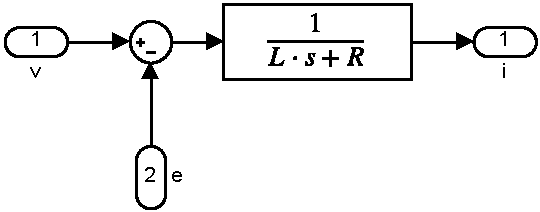
\includegraphics[]{./fig/fig1.pdf}
    \caption{ACサーボモータの電気的モデル}
\end{figure}

\subsubsection{機械的モデル}
 トルク$\tau(s)$と負荷トルク$\tau_l(s)$を入力すると速度$\omega(s)$が出力される機械的モデルは以下の式および図で表される.
\begin{equation}
    \omega(s) = \frac{1}{Js + D}\left(\tau(s) - \tau_l(s)\right)
\end{equation}

\begin{figure}[H]
    \centering
    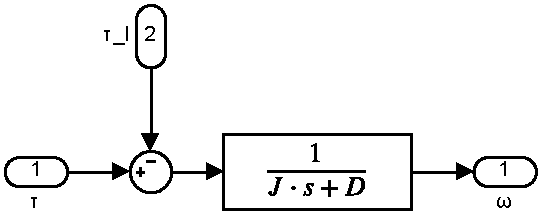
\includegraphics[]{./fig/fig2.pdf}
    \caption{ACサーボモータの機械的モデル}
\end{figure}

\subsubsection{モデルの統合}
 以上でACサーボモータの電気的モデルと機械的モデルを構築できたので,これを組み合わせて,最終的なACサーボモータのモデルを完成させる.\\
 電気的モデルの出力は$i(s)$,機械的モデルの入力は$\tau(s)$であり,単位が異なる.しかし,モータに流れる電流と発生するトルクには比例関係があるため,$\tau(s) = K_t i(s)$と表せる.この$K_t$[Nm/A]をトルク定数と呼ぶ.\\
 また,モータの速度と逆起電力にも比例関係があるため,$e(s) = K_e \omega(s)$と表される.この$K_e$[V/(rad/s)]を誘起電圧定数と呼ぶ.\\
 これらを踏まえて, ACサーボモータ全体のモデルはFig.3のようになる.
\begin{figure}[H]
    \centering
    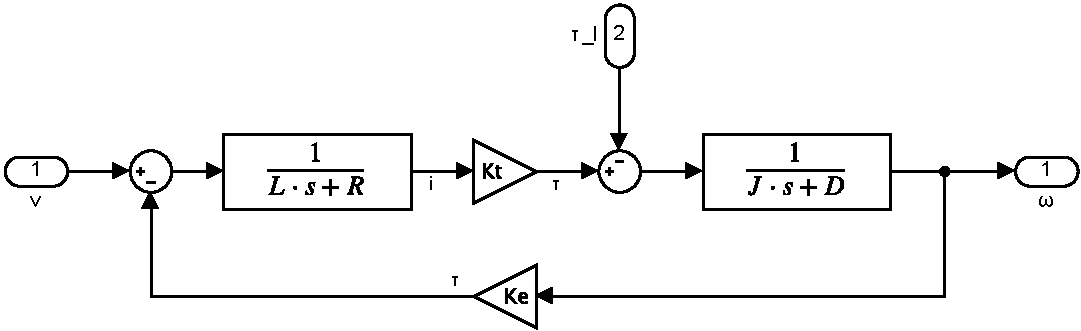
\includegraphics[width=15cm]{./fig/fig3.pdf}
    \caption{ACサーボモータ全体のモデル}
\end{figure}

\subsection{制御器の設計}
 前項でACサーボモータのモデルを構築できたので,次にモータの位置制御器の設計を行う.ACサーボモータの位置制御系は,内側から「電流制御系」,「速度制御系」,「位置制御系」の3重の制御ループで構成されるのが一般的である.\\
 まずは電流制御について考える.電流制御系はFig.4のようなブロック図で表される.なお,$i^{ref}$は目標の電流値である.
\begin{figure}[H]
    \centering
    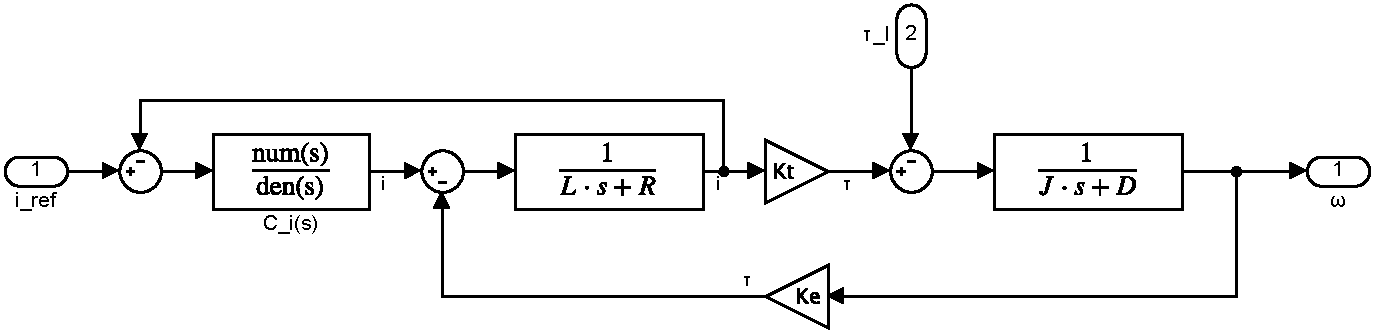
\includegraphics[width=15cm]{./fig/fig4.pdf}
    \caption{ACサーボモータの電流制御系のブロック図}
\end{figure}

\subsubsection{電流制御}
 ACサーボモータ制御の究極的な目的は位置制御や速度制御であるにも関わらず電流制御をする意図は,モータのモデルを簡単にするためである.電流制御が正常に行われていれば,実電流は目標の電流値に必ず追従する.したがって,電流制御をかけられたモータのブロック図はFig.5のような簡単なモデルに書き換えらる.
\begin{figure}[H]
    \centering
    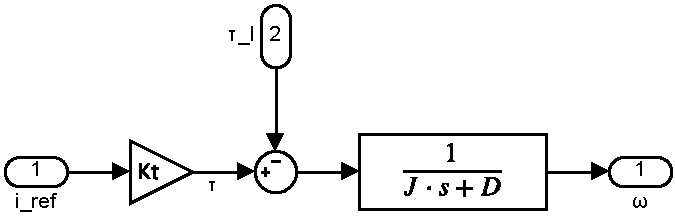
\includegraphics[]{./fig/fig5.pdf}
    \caption{電流制御をかけられたモータのブロック図}
\end{figure}

\subsubsection{速度制御}
続いて,速度制御について考える.速度制御系はFig.6のようなブロック図で表される.なお,$\omega^{ref}$は目標の速度である.
\begin{figure}[H]
    \centering
    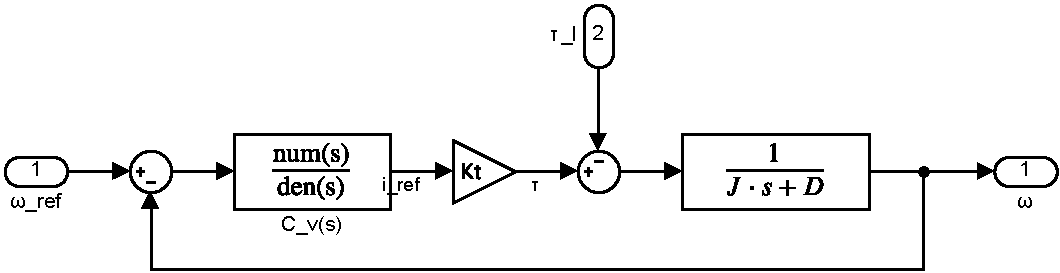
\includegraphics[width=15cm]{./fig/fig6.pdf}
    \caption{ACサーボモータの速度制御系のブロック図}
\end{figure}

 この時の速度制御器$C_v(s)$について検討する.\\
 まずは$C_v(s)$をP制御にした場合を考察する.速度P制御の際,目標値伝達関数はEqn(3)となる(導出は課題3で行なっている).
\begin{equation}
    \frac{\omega}{\omega^{ref}} = \frac{K_{pv} K_t}{Js + D + K_{pv} K_t}
\end{equation}

 このとき,ステップ応答において,モータの速度が最終的にどのような値に落ち着くのかを最終値の定理より求める.
\begin{eqnarray}
    \lim_{s \to 0} s \frac{\omega(s)}{\omega^{ref}(s)} \frac{1}{s} &=& \frac{K_{pv} K_t}{Js + D + K_{pv} K_t}\nonumber \\
    &=& \frac{K_{pv} K_t}{D + K_{pv} K_t} \nonumber \\
    &\neq& 1
\end{eqnarray}

 このことから,速度P制御では定常偏差が発生し,目標値に到達できないことがわかる.

 次に$C_v(s)$をPI制御にした場合を考察する.速度PI制御の際,目標値伝達関数はEqn(5)となる(導出は課題3で行なっている).
\begin{equation}
    \frac{\omega}{\omega^{ref}} = \frac{K_{pv}K_ts + K_{iv}}{Js^2 + \left(D+K_tK_{pv}\right)s + K_{iv}}
\end{equation}

 このとき,ステップ応答において,モータの速度が最終的にどのような値に落ち着くのかを最終値の定理より求める.
\begin{eqnarray}
    \lim_{s \to 0} s \frac{\omega(s)}{\omega^{ref}(s)} \frac{1}{s} &=& \lim_{s \to 0} \frac{K_{pv}K_ts + K_{iv}}{Js^2 + \left(D+K_tK_{pv}\right)s + K_{iv}} \nonumber \\
    &=& \frac{K_{iv}}{K_{iv}} \nonumber \\
    &=& 1
\end{eqnarray}
 目標値伝達関数が1(ステップ応答の目標値)に収束することがわかる.\\


\subsubsection{位置制御}
 最後に位置制御について考える.位置制御系はFig.7のようなブロック図で表される.なお,$\theta^{ref}$は目標の位置である.
\begin{figure}[H]
    \centering
    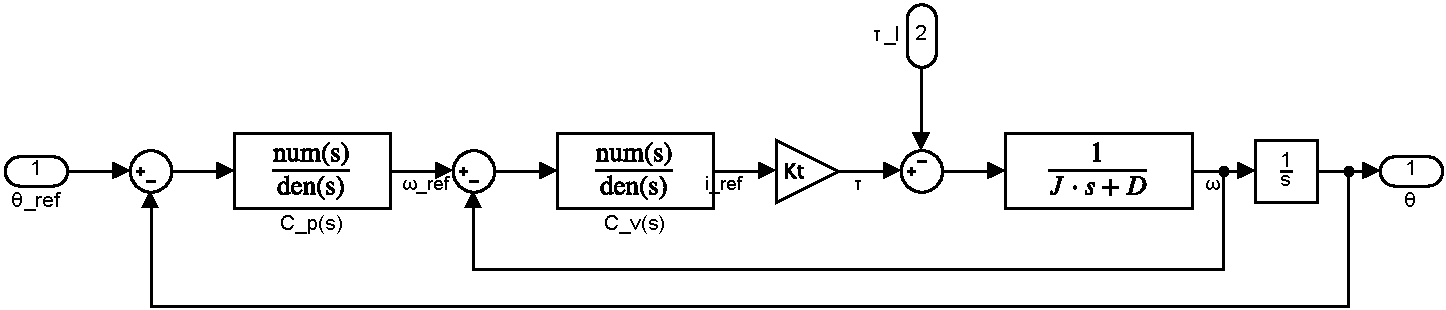
\includegraphics[width=15cm]{./fig/fig7.pdf}
    \caption{ACサーボモータの位置制御系のブロック図}
\end{figure}

 この時の速度制御器$C_p(s)$について検討する.$C_p(s)$をP制御とした時,目標値伝達関数はEqn(7)となる.
\begin{equation}
    \frac{\theta}{\theta^{ref}} = \frac{C_v(s) K_t K_{pp}}{Js^2 + \left(D + C_v(s) K_t\right)s + C_v(s) K_t K_{pp}}
\end{equation}

 このとき,ステップ応答において,モータの速度が最終的にどのような値に落ち着くのかを最終値の定理より求める.
\begin{eqnarray}
    \lim_{s \to 0} s \frac{\theta}{\theta^{ref}} \frac{1}{s} &=& \lim_{s \to 0} \frac{C_v(s) K_t K_{pp}}{Js^2 + \left(D + C_v(s) K_t\right)s + C_v(s) K_t K_{pp}} \nonumber \\
    &=& \frac{C_v(s) K_t K_{pp}}{C_v(s) K_t K_{pp}} \nonumber \\
    &=& 1
\end{eqnarray}
 目標値伝達関数が1(ステップ応答の目標値)に収束するため,位置制御においてはP制御で十分であると言える.\\

\section{課題2:下図の電流指令$i^{ref}$から速度$\omega$までの伝達関数と,電流指令$i^{ref}$から位置$\theta$までの伝達関数を求めよ.}
\begin{figure}[H]
    \centering
    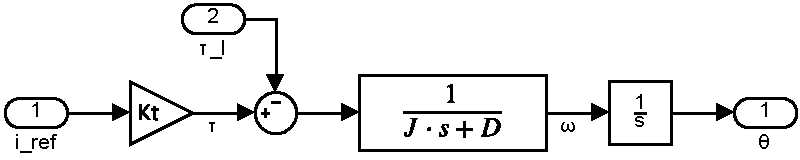
\includegraphics[]{./fig/2.pdf}
    \caption{課題2}
\end{figure}

 $\tau_l$ = 0として考えると,伝達関数はEqn(9)のようになる.
\begin{eqnarray}
\theta &=& i^{ref} \cdot K_t \cdot \frac{1}{Js+D} \cdot \frac{1}{s} \nonumber \\
\frac{\theta}{i^{ref}} &=& \frac{Kt}{Js^2 + Ds}
\end{eqnarray}

 よって,Fig.8をまとめると,Fig.9のようになる.
\begin{figure}[H]
    \centering
    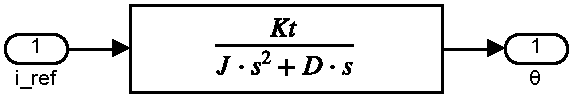
\includegraphics[]{./fig/2_ans.pdf}
    \caption{課題2のブロック図をまとめたブロック図}
\end{figure}


\section{課題3:P速度制御系とPI速度制御系の速度指令$\omega^{ref}$から速度$\omega$までと,負荷トルク$\tau_l$から速度$\omega$までのそれぞれ2つの伝達関数を求めよ.}
\begin{figure}[H]
    \centering
    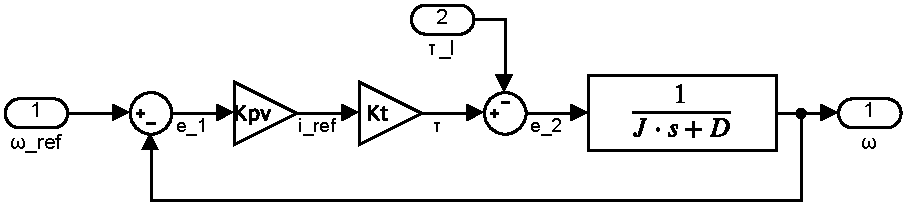
\includegraphics[]{./fig/3_P.pdf}
    \caption{課題3:P速度制御系}
\end{figure}
\begin{figure}[H]
    \centering
    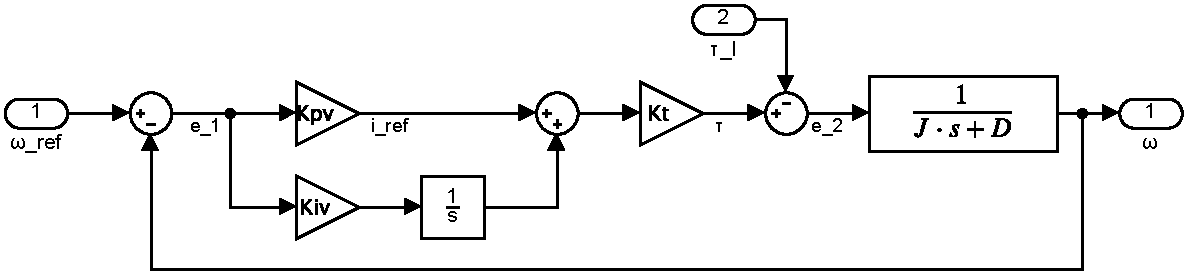
\includegraphics[width=15cm]{./fig/3_PI.pdf}
    \caption{課題3:PI速度制御系}
\end{figure}

 まず,P速度系の速度司令から速度の伝達関数を求める.$\tau_l$ = 0,$\omega^{ref}$と出力の減算点を$e_1$として$e_1$を表すと
\begin{eqnarray}
    e_1 &=& \omega^{ref} - e \cdot K_{pv} \cdot K_t \cdot \frac{1}{Js + D} \nonumber \\
    e_1 + e \cdot K_{pv} \cdot K_t \cdot \frac{1}{Js + D}&=& \omega^{ref}  \nonumber \\
    e_1 \left(1 + \frac{K_{pv} K_t}{Js + D} \right) &=& \omega^{ref}  \nonumber \\
    e_1 &=& \dfrac{\omega^{ref}}{1 + \dfrac{K_{pv} K_t}{Js + D}}  \nonumber \\
    e_1 &=& \frac{\omega^{ref}\left(Js+D\right)}{Js + D + K_{pv} K_t}  \nonumber
\end{eqnarray}

 これを元に$\omega$を求めると
\begin{eqnarray}
    \omega &=& e_1 \cdot \frac{K_{pv} K_t}{Js + D} \nonumber \\
           &=& \frac{\omega^{ref}\left(Js+D\right)}{Js + D + K_{pv} K_t} \cdot \frac{K_{pv} K_t}{Js + D} \nonumber \\
           &=& \frac{K_{pv} K_t}{Js + D + K_{pv} K_t} \cdot \omega^{ref}\nonumber
\end{eqnarray}

 よって,伝達関数はEqn(10)となる
\begin{equation}
    \frac{\omega}{\omega^{ref}} = \frac{K_{pv} K_t}{Js + D + K_{pv} K_t}
\end{equation}

\begin{figure}[H]
    \centering
    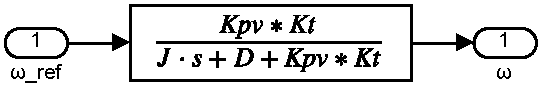
\includegraphics[]{./fig/3_P_ans.pdf}
    \caption{課題3:P速度制御系の速度司令から速度をまとめたブロック図}
\end{figure}

 次にPI速度系の速度司令から速度の伝達関数を求める.Eqn(10)において$K_{pv}$を$K_{pv}+\frac{K_{iv}}{s}$と置き換えると求められる.
\begin{eqnarray}
    \frac{\omega}{\omega^{ref}} &=& \dfrac{\left(K_{pv}+\dfrac{K_{iv}}{s}\right)  K_t}{Js + D + \left(K_{pv}+\dfrac{K_{iv}}{s}\right) K_t} \nonumber \\
                                &=& \frac{K_{pv}K_ts + K_{iv}}{Js^2 + \left(D+K_tK_{pv}\right)s + K_{iv}}
\end{eqnarray}

\begin{figure}[H]
    \centering
    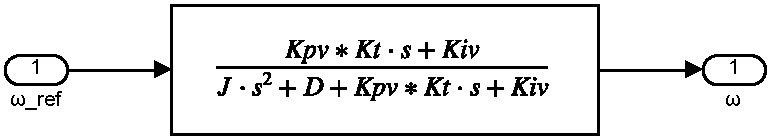
\includegraphics[]{./fig/3_PI_ans.pdf}
    \caption{課題3:PI速度制御系の速度司令から速度をまとめたブロック図}
\end{figure}

 続いてP制御系における負荷トルクから速度までの伝達関数を求める.$\omega_l$ = 0,$K_t$の出力と$\tau_l$の減算点を$e_2$として$e_2$を表すと
\begin{eqnarray}
    e_2 &=& e_2 \cdot - \left(\frac{K_{pv}K_t}{Js + D}\right) -\tau_l \nonumber \\
    e_2\left(1 + \frac{K_{pv}K_t}{Js + D}\right) &=& -\tau_l \nonumber \\
    e_2 &=& -\dfrac{\tau_l}{1 + \dfrac{K_{pv}K_t}{Js + D}} \nonumber
\end{eqnarray}

 これを元に$\omega$を求めると
\begin{eqnarray}
    \omega &=& e_2 \cdot \frac{1}{Js + D} \nonumber \\
           &=& -\dfrac{\tau_l}{1 + \dfrac{K_{pv}K_t}{Js + D}} \cdot \frac{1}{Js + D} \nonumber \\
           &=& -\frac{\tau_l}{Js + D + K_{pv}K_t} \nonumber
\end{eqnarray}

 よって,伝達関数はEqn(12)となる
\begin{equation}
    \frac{\omega}{\tau_l} = -\frac{1}{Js + D + K_{pv}K_t}
\end{equation}

\begin{figure}[H]
    \centering
    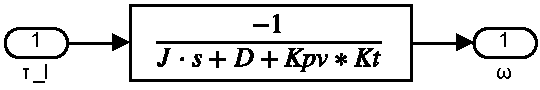
\includegraphics[]{./fig/3_P_tau_ans.pdf}
    \caption{課題3:P速度制御系の負荷トルクから速度をまとめたブロック図}
\end{figure}

 最後にPI速度系の負荷トルクから速度の伝達関数を求める.Eqn(12)において$K_{pv}$を$K_{pv}+\frac{K_{iv}}{s}$と置き換えると求められる.
\begin{eqnarray}
    \frac{\omega}{\tau_l} &=& -\dfrac{1}{Js + D + \left(K_{pv}+\dfrac{K_{iv}}{s}\right)K_t} \nonumber \\
                          &=& -\dfrac{1}{Js + D + K_{pv}K_t + \dfrac{K_{iv}K_t}{s}} \nonumber \\
                          &=& -\dfrac{s}{Js^2 + \left(D + K_{pv}K_t\right)s + K_{iv}K_t}
\end{eqnarray}

\begin{figure}[H]
    \centering
    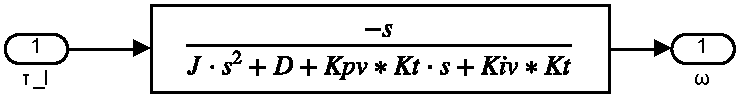
\includegraphics[]{./fig/3_PI_tau_ans.pdf}
    \caption{課題3:PI速度制御系の負荷トルクから速度をまとめたブロック図}
\end{figure}

\section{課題4:PI制御器を双一次変換せよ.}
 Fig.16のようなPI制御器の双一次変換を考える.
\begin{figure}[H]
    \centering
    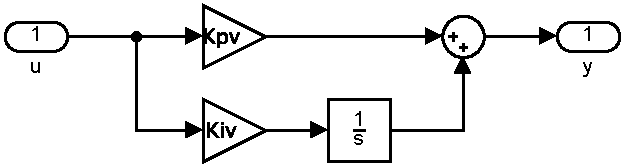
\includegraphics[]{./fig/4.pdf}
    \caption{課題4:PI制御器のブロック図}
\end{figure}

 入力$u$と出力$y$の関係は
\begin{eqnarray}
    y &=& \left(K_{pv} + \frac{K_{iv}}{s} \right) \cdot u \nonumber \\
      &=& K_{pv} \cdot u + K_{iv} \cdot u \cdot \frac{1}{s}
\end{eqnarray}

 Eqn(14)において$s$を$\frac{2}{T} \cdot \frac{1-z^2}{1+z^2}$と置き換えて双一次変換を行うと
\begin{eqnarray}
    y &=& K_{pv} \cdot u + K_{iv} \cdot \frac{T}{2} \cdot \frac{1+z^2}{1-z^2} \nonumber \\
    y (1-z^2) &=& K_{pv}u(1-z^2) + \frac{T}{2} K_{iv} u (1+z^2) \nonumber \\
    y - yz^2 &=& K_{pv}(u - uz^2) + \frac{T}{2} K_{iv} (u + uz^2) \nonumber \\
    y &=& K_{pv}(u - uz^2) + \frac{T}{2} K_{iv} (u + uz^2) + yz^2
\end{eqnarray}


\section{課題5:換算式について}
\subsection{換算式Aについて:5Vのアナログ電圧信号を入力すると9.6Aの電流をモータに流すように作られている.電流指令[A]から電圧値[V]に変換する式を作れ.}
 変換式の入出力関係はTable1のようになる.
\begin{table}[hbtp]
    \caption{電流指令$i^{ref}$[A]から電圧値$v$[V]への変換式の入出力関係}
    \centering
    \begin{tabular}{cc}
    \hline
    入力(電流指令$i^{ref}$[A])  & 出力(電圧値$v$[V]) \\
    \hline \hline
    +9.6 & 5  \\
    0    & 0  \\
    \hline
    \end{tabular}
\end{table}

 入出力の関係が線形であると仮定して,Table1にしたがって電流指令$i^{ref}$[A]から電圧値$v$[V]に変換する式を組み立てると.次のようになる($v_1 = 0$,$v_2 = 5$,$i^{ref}_1 = 0$,$i^{ref}_2 = 9.6$).

\begin{eqnarray}
    v - v_1 &=& \frac{v_2 - v_1}{i^{ref}_2 - i^{ref}_1} \cdot \left(i^{ref} - i^{ref}_1 \right) \nonumber \\
    v - 0 &=& \frac{5 - 0}{9.6 - 0}\cdot \left(i^{ref} - 0 \right) \nonumber \\
    v  &=& \frac{5}{9.6}i^{ref}
\end{eqnarray}


\subsection{換算式Bについて:アナログ信号の最大電圧振幅は$\pm$5Vである.所望の電圧値[V]からD/A変換器に入力すべき整
数値(10進数)に変換する式を作れ.}
 変換式の入出力関係はTable2のようになる.
\begin{table}[hbtp]
    \caption{所望の電圧値$v$[V]から入力すべき整数値Nへの変換式の入出力関係}
    \centering
    \begin{tabular}{cc}
    \hline
    入力(所望の電圧値$v$[V])  & 出力(入力すべき整数値N) \\
    \hline \hline
    +5 & 65535  \\
    -5 & 0 \\
    \hline
    \end{tabular}
\end{table}

 入出力の関係が線形であると仮定して,Table2にしたがって所望の電圧値$v$[V]から入力すべき整数値Nに変換する式を組み立てると.次のようになる($N_1 = 0$,$N_2 = 65535$,$v_1 = -5$,$v_2 = 5$).

\begin{eqnarray}
    N - N_1 &=& \frac{N_2 - N_1}{v_2 - v_1} \cdot \left(v - v_1 \right) \nonumber \\
    N - 0 &=& \frac{65535 - 0}{5 - (-5)} \cdot \left(v - (-5) \right) \nonumber \\
    N &=& \frac{65535}{10} \cdot \left(v + 5 \right)
\end{eqnarray}

\section{課題6:インクリメンタルロータリエンコーダについて、モータ位置が0[rad]から2$\pi$[rad]まで回転すると8000パルスが出力され、エンコーダカウンタの整数値は0から8000に増加する.エンコーダカウンタの整数値からモータ位置[rad]に変換する式
を作れ.}
 変換式の入出力関係はTable3のようになる.
\begin{table}[hbtp]
    \caption{エンコーダカウンタの整数値$N_{cnt}$からモータ位置$\theta$[rad]への変換式の入出力関係}
    \centering
    \begin{tabular}{cc}
    \hline
    入力(エンコーダカウンタの整数値$N_{cnt}$)  & 出力(モータ位置$\theta$[rad]) \\
    \hline \hline
    8000 & 2$\pi$  \\
    0 & 0 \\
    \hline
    \end{tabular}
\end{table}

 入出力の関係が線形であると仮定して,Table3にしたがってエンコーダカウンタの整数値$N_{cnt}$からモータ位置$\theta$[rad]に変換する式を組み立てると.次のようになる($\theta_1 = 0$,$\theta_2 = 2\pi$,$N_{cnt_1} = 0$,$N_{cnt_2} = 8000$).

\begin{eqnarray}
    \theta - \theta_1 &=& \frac{\theta_2 - \theta_1}{N_{cnt_2} - N_{cnt_1}} \cdot \left(N_{cnt} - N_{cnt_1} \right) \nonumber \\
    \theta - 0 &=& \frac{2\pi - 0}{8000 - 0} \cdot \left(N_{cnt} - 0 \right) \nonumber \\
    \theta &=& \frac{2\pi}{8000} \cdot N_{cnt}
\end{eqnarray}

\end{document}



